\subsection{Attēlu raksturpunktu salāgošanas algoritmi} \label{sec:matching}
\begin{figure}[tbh]
	\centering
	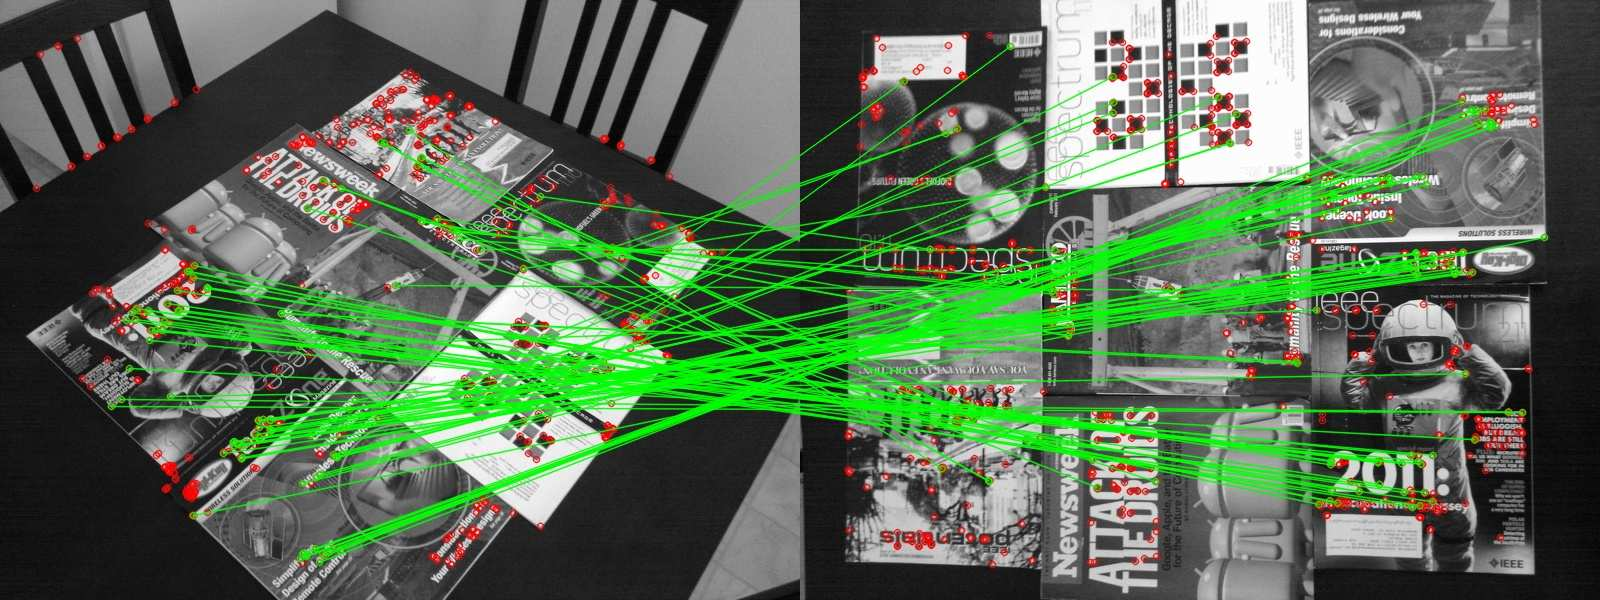
\includegraphics[width=0.8\textwidth]{orb-match}
	\caption{Attēlu pāra raksturpunktu salāgošana ar ORB~\cite{ORB}.}
	\label{fig:orb}
\end{figure}

Raksturpunktu salāgošana ir punktu pāru (vai kopu) atrašana divos
(vai vairākos) attēlos, kuri atbilst vienam un tam pašam attēlā redzamam
objektam. Salāgošanas piemērs redzams \ref{fig:orb}~attēlā, kur ar zaļu
savienoti salāgotie raksturpunktu pāri un ar sarkanu apzīmēti raksturpunkti,
kuriem pāris nav atrasts.

Raksturpunktu salāgošana tiek izmantota tādos mašīnredzes pielietojumos, kā
% TODO: citēt pielietojumus
objektu atpazīšanā un sekošanā, attēlu ,,sašūšanā'', 
telpiskās informācijas rekonstrukcijā (kartēšanā) no attēliem,
vienlaicīgā pašlokalizācijā un kartēšanā (SLAM), u.c..

\TODO


